\section{Hardware design} \label{chap:hardware}

In this section, the hardware design and implementation of the micromouse robot are described. First, the corresponding electrical circuit, known as scematic, is broken down to its components and thoroughly presented. In the next subsection, the actual components chosen for the hardware implementation are listed. The model for the final Printed Circuit Board (PCB) follows right after, where the chosen electrical components are placed in the computer model. Last, but not least, the protective casing for the micromouse is described.

\vspace{1cm}

\subsection{Schematic and Components Description}

The first step in the development of the hardware is the drawing of the electrical circuit. The realization of a moving micromouse demands for the combination of a variety of components connected to each other. Exactly this is described in the so called schematic of the circuit, which resembles a drawing on paper. 
The schematic of the micromouse can be seen in Fig. \ref{fig:schematic_overview}.

\begin{figure}[htb]
    \centering
    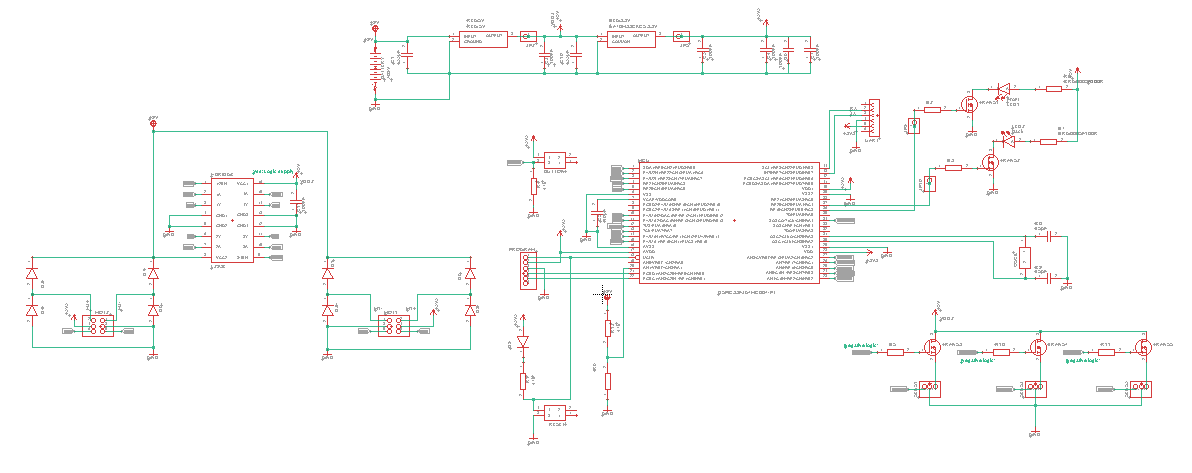
\includegraphics[width=1\textwidth]{figures/hardware/Schematic.PNG}
    \caption{Schematic overview of the micromouse}
    \label{fig:schematic_overview}
\end{figure}

This can look intimidating at first and definitely not readable in such a miniature picture. So, let's break it down to its components and describe its sub-circuits.

With the exception of the first subsection, the components will be presented from left to right and from top to bottom, so that the reader may always refer to the overview schematic to get a clear picture of a component's relation to the whole.

\FloatBarrier
\vspace{1cm}

\subsubsection{Microcontroller (MCU)}

The microcontroller (mcu) can be seen in Fig. \ref{fig:mcuL}.
Notice that the symbolic representation of the mcu, specifically when it comes to the location of its pins, doesn't correspond to the real model. For the purpose of the schematic, we don't really care about the real location of the pins. As will be seen later, this becomes of importance when placing the components on the board to be printed.

\begin{figure}[htb]
    \centering
    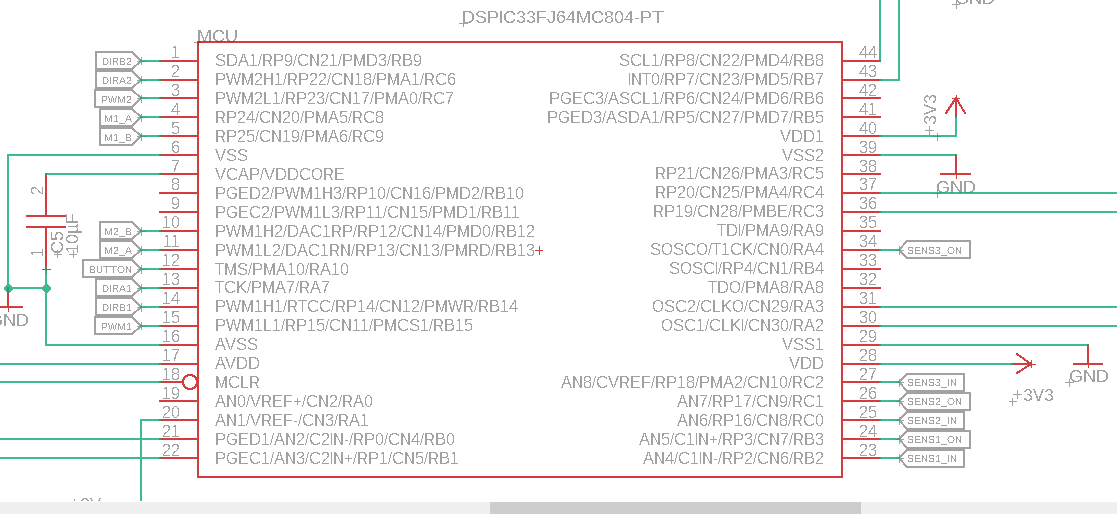
\includegraphics[width=0.8\textwidth]{figures/hardware/MCU.PNG}
    \caption{The dsPIC33FJ64MC804 microcontroller}
    \label{fig:mcuL}
\end{figure}

\FloatBarrier

The assignment of mcu pins to components is presented in the Software Section and will not be repeated here. Please refer to that Section for understanding the functionality of its pin in our circuit.

Another point to notice about the pin connections is the convenient label feature that Eagle offers. Notice how some of the components are wired to the pins of the mcu, while other connections are represented as labels. Labels in the circuit are the equivalent of wires and greatly contribute to the readability and modularity of the schematic. As long as two wires anywhere in the circuit share the same label, they are connected.

A last comment has to be made about the pins of the mcu: The pins, as everything in our circuit, are very real components and therefore are subject to electrical limitations. This is a very important point to keep in mind, when driving any load, such as LEDs or a motor, but also when connecting input signals, such as sensors.
Specifically, in the section "Electrical Characteristics" in \cite{mcu}, we find maximum values for individual pins and for all utilized pins combined. These can be seen in Fig. \ref{fig:electrical}. These characteristics lead to some important design decisions, specifically named in later subsections.

\begin{figure}[htb]
    \centering
    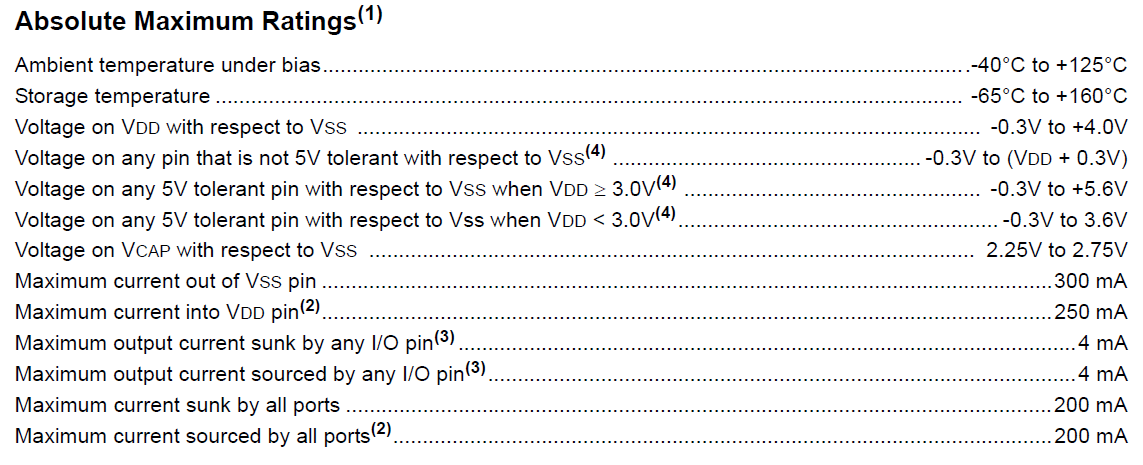
\includegraphics[width=0.8\textwidth]{figures/hardware/Electrical.PNG}
    \caption{Electrical limitations for the pins of the mcu}
    \label{fig:electrical}
\end{figure}

\FloatBarrier
\vspace{1cm}

\subsubsection{Votage Regulators}

The necessity for voltage regulators, which can be seen in Fig. \ref{fig:battery}, arises from the need for different voltages present in our system. 
Specifically, as found in \cite{mcu}, the mcu considers 3.3V as logical one and it is this voltage we need to provide to it (see VDD pins). The distance sensors used (taken from a previous micromouse model) need 5V. And yet the motors need 6V, as can be seen in \cite{motor}. 
Notice that we are using a battery of 9V. Therefore, we need a way to generate the required 3 different voltages.

\begin{figure}[htb]
    \centering
    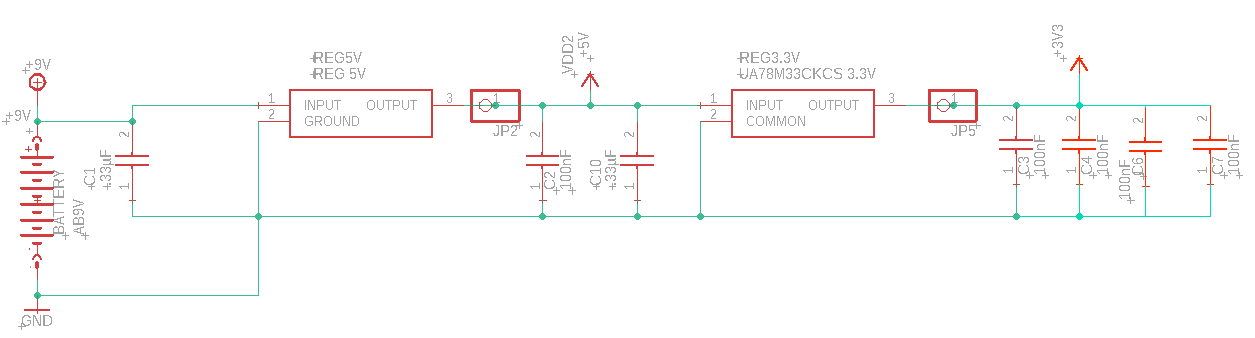
\includegraphics[width=0.8\textwidth]{figures/hardware/VoltageandCapacitors.PNG}
    \caption{The battery and voltage regulators}
    \label{fig:battery}
\end{figure}

\FloatBarrier

When it comes to the motor, we can regulate the voltage we feed it with, by regulating the maximum duty cycle of the PWM (explained in another Section). So, we provide it with a fraction of the available 9V.
For the distance sensors and the mcu, 2 voltage regulators are used in succession. They provide our components with steady voltage, necessary for functioning properly.

Now, notice the capacitors used in Fig. \ref{fig:battery}. Capacitors are used in the input and output of the voltage regulators. Additionally, a bunch of capacitors can be observed at the far right part of the sub-circuit.

All of these capacitors have both a special name and function. They are called decoupling capacitors and their role is to help in providing steady voltage. Specifically, they are always physically connected close to their corresponding component and should a temporary lack of electrons happen, they provide from their surplus, keeping the voltage steady.
The capacitors at the far right are only symbolically placed there in the circuit. In reality, they are connected between the pins of the mcu that connect to VDD (3.3V) and ground (GND). Every decoupling capacitor is ideally connected as close to the actual component pins as possible, as will be later seen in the PCB Section. The values of the capacitors are dictated by the datasheets of the specific components used. For example, have a look in \cite{mcu}.

\vspace{1cm}


\subsubsection{H-bridge and Motors}

Next, the motors and H-bridge sub-circuit will be presented. 
First, let us consider the motors. As can be seen in Fig. \ref{fig:motors}, the motors are symmetrically connected to the H-bridge and to the mcu. So, let us concentrate on one of them, the left. The same explanation applies for the other one.

\begin{figure}[htb]
    \centering
    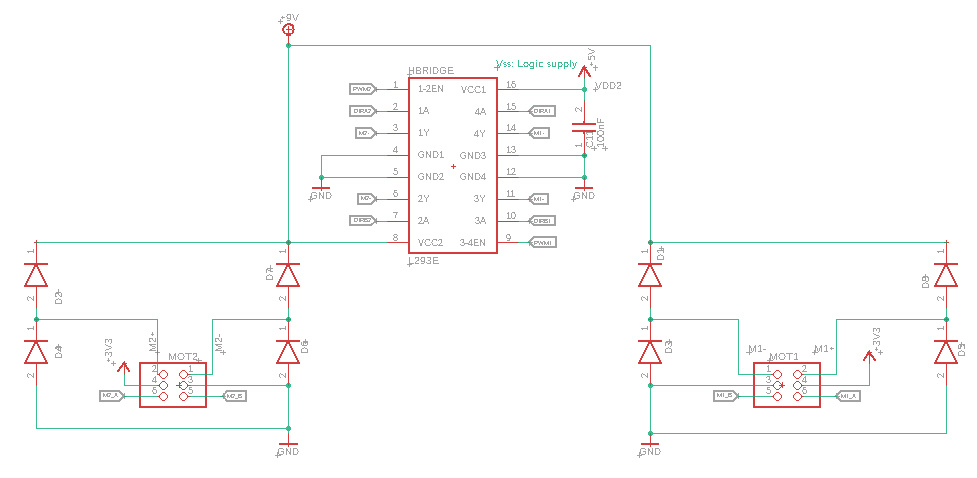
\includegraphics[width=0.8\textwidth]{figures/hardware/MotorsandHBridge.PNG}
    \caption{The motors and the H-bridge}
    \label{fig:motors}
\end{figure}

\FloatBarrier

In Fig. \ref{fig:motorPins} taken from the motor datasheet, the motor pins can be noticed. 
One pair of pins (1, 2) refers to the voltage we feed to the motor. Remember that we are using PWM (max 6V) to control how fast the motor turns and notice that if the voltage is reversed, the rotation of the motor is also reversed. As we will shortly see, for this purpose, the H-bridge is needed. The function of reversing the motor's rotation is hihgly desirable, since we want our 2-wheels micromouse to be able to move backwards and to turn on spot (imagine one wheel moving to one direction and the other to the opposite direction with the same velocity).

\begin{figure}[htb]
    \centering
    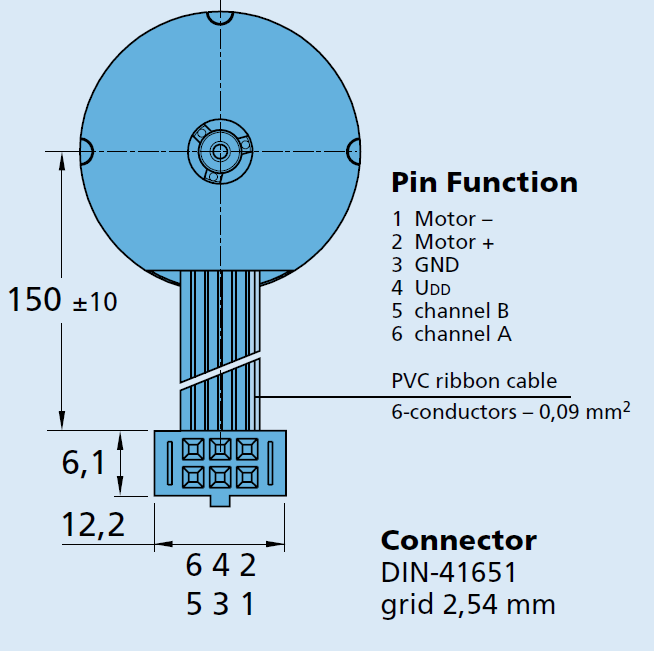
\includegraphics[width=0.8\textwidth]{figures/hardware/motor.PNG}
    \caption{The motor pins as presented in its datasheet}
    \label{fig:motorPins}
\end{figure}

\FloatBarrier

Another pair of pins (3, 4) refers to the voltage feed of the motor encoder. And the last pair of pins (5, 6) are used for the output of the motor encoder signals. These signals encode the motor's rotational position every moment and are fed to the mcu. In the mcu, with the help of the quadrature encoder (QE) module, they can be translated to real position in space.

Finally, let us consider the H-bridge. As mentioned, the need for the H-bridge arises from the function of reversing the motor polarity and thus its rotation. Without the use of an H-bridge, one would have to physically reverse the wires for the motor feed. If it is impractical with the use of wires, it is impossible with the tracks on a PCB. Instead, the H-bridge can conveniently reverse the voltage. First, have a look at the exemplary circuit in Fig. \ref{fig:HData}, take from the datasheet of the H-bridge \cite{Hbridge}.

\begin{figure}[htb]
    \centering
    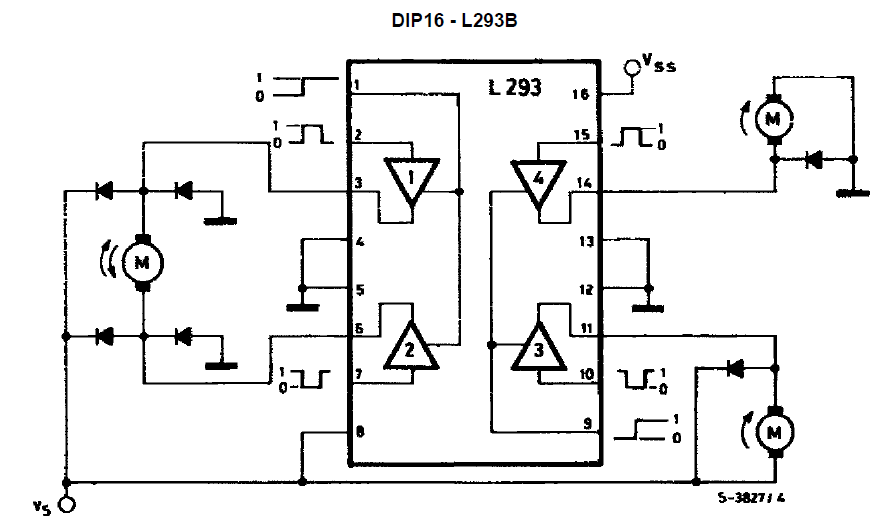
\includegraphics[width=0.8\textwidth]{figures/hardware/HbridgeDatasheet.PNG}
    \caption{Exemplary motor connection from the H-bridge datasheet}
    \label{fig:HData}
\end{figure}

\FloatBarrier

We feed our PWM in pin 1. Pins 2 and 7 are used for controlling the direction of rotation of the motor. The truth table is simple: If one direction pin is 1 and the other 0, then the logical 1 defines the direction. If both of the pins are set to logical 0 or 1, the motor breaks. Notice how the pins 3 and 6 feed the voltage to the motor and are coupled with the direction pins.

As a last comment, in both Fig. \ref{fig:HData} and Fig. \ref{fig:motors} notice the existence of diodes. Again, these diodes have both a special name and a special function. They are called \textit{catch diodes} and to understand their use, please refer to \cite{catchDiodes}, where a beginners-friendly introduction to H-bridges is offered.

For our purposes, it suffices to say that the presence of catch diodes is necessary for the smooth functioning of our brushed motor. Consider the case, when the motor changes direction or stops from spinning. In order for this to happen, the internal switches of the H-bridge need to open (remember the direction pins). Temporarily, the current that was flowing in the circuit through the motor has to go ("escape") somewhere, since due to the inductance nature of the motor, the current cannot instantly go to zero . It is not a good idea to dissipate the current through our H-bridge pins/ switches, without an alternative: The current will try to jump an open switch, creating a spark and probably burning the pin/ switch. The catch diodes provide this alternative: The current flows through them in a forward manner and is returned to the source.

\vspace{1cm}


\subsubsection{Extra Button}

Naturally, the more input options we have for our micromouse robot, the more flexible the commands we can issue and the more complicated the software can be. Therefore, we added a button (switch), which can be seen in Fig. \ref{fig:button}.

\begin{figure}[htb]
    \centering
    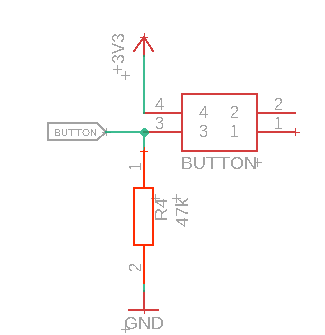
\includegraphics[width=0.8\textwidth]{figures/hardware/Button.PNG}
    \caption{An extra button for input}
    \label{fig:button}
\end{figure}

\FloatBarrier

A typical pull-down resistor of 47k is used, to make sure the mcu pin never has an undefined logical value ("floating"). When it comes to the resistance value, it is somewhat arbitrary in that it does its job. A different value could have been selected.
For the current that flows through the resistor, when the button is pressed, we have:

$$V = I*R => 3.3 = I*47 => I = 0.07mA$$

If a much smaller value for the resistance was used, then the current would be much larger, leading to unnecessary power dissipation on the resistance and heating. Also, in this case, there is the possibility for the input to the mcu pin to be stuck in a low, logical 0 level, no matter if the button is pressed or not.

\vspace{1cm}


\subsubsection{Programmer}

The programmer is the device that allows for (re)programming of the mcu. The way it is connected is rather straightforward and can be seen in Fig. \ref{fig:programmer}.

\begin{figure}[htb]
    \centering
    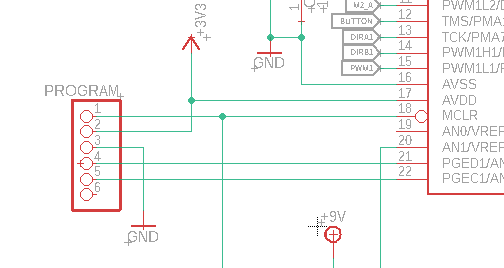
\includegraphics[width=0.8\textwidth]{figures/hardware/Programmer.PNG}
    \caption{The programmer}
    \label{fig:programmer}
\end{figure}

\FloatBarrier
\vspace{1cm}


\subsubsection{Reset Button}

A reset button is needed in case something goes wrong during the execution of the program in the mcu, or if one simply needs to start the execution from the start again. Notice that the MCLR (Master Clear) pin is also used by the programmer for programming and debugging, as can be found in \cite{mcu}.

The reset activation logic in our mcu is negative or inverse, as can be seen in Fig. \ref{fig:reset}. A diode and a pull-up resistor (similar to the pull-down used for the other button) connect the voltage feed to the mcu. Once the button is pressed, a connection with the ground is made and the mcu is reset.
Again the choice of the resistance value is a bit arbitrary.

\begin{figure}[htb]
    \centering
    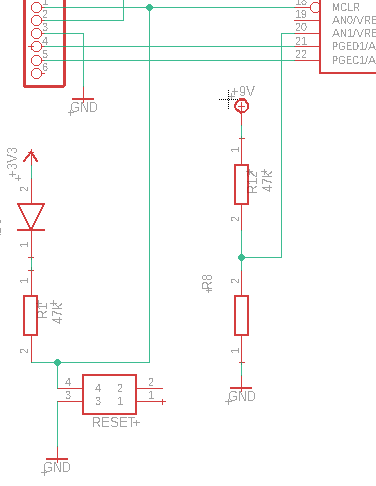
\includegraphics[width=0.8\textwidth]{figures/hardware/MCLRandBatteryMeasurement.PNG}
    \caption{The reset button and the battery voltage measurement circuit}
    \label{fig:reset}
\end{figure}

\FloatBarrier
\vspace{1cm}


\subsubsection{Battery Measurement}

In an ideal world, our battery would provide steadily 9V until its exhaustion. However, this is not the case. As the battery is depleted, the voltage it provides is reduced. It would be useful to know exactly how much voltage the battery provides at any given point in time. Feeding this value to the mcu, we can take decisions accordingly. For example, we can regulate the PWM maximum duty cycle value to keep the motor spinning at its maximum velocity, even though the battery is depleted. Remember that our motor can take a maximum of 6V for its fastest performance.

In order to realize such a schema, a simple voltage divider sub-circuit and an analog pin of the mcu can be used, as can be seen in the above Fig. \ref{fig:programmer}.
In order to keep the amount of different components to a minimum, a resistance of 47k is used. The question now is, what should the value of the other resistance be, in order for the input voltage to the mcu to be 3.3V for a 9V battery. 

If we call the unknown resistor R8, as in the figure, we can use the known equation for a voltage divider:

$$V_{MCU} = \frac{R_8}{47+R_8} * 9V = 3.3V$$

With a value of $ R_8 = 22k $, we can easily calculate the resulting $V_{MCU} = 2.87V$. This is a convenient value, since for example another battery of higher voltage, e.g. 10V, could be used. By choosing this value we fulfill our initial purpose and have some flexibility for higher voltages.

\vspace{1cm}

\subsubsection{Universal Asynchronous Communication (UART)}


Despite us building an autonomous micromouse robot that can navigate in a labyrinth, we would still like to be able to issue stand-alone commands via UART. Hence, the UART sub-circuit of Fig. \ref{fig:uart}. The connection is straight-forward. Only attention is required in connecting RX to TX of the mcu and vice-versa.

\begin{figure}[htb]
    \centering
    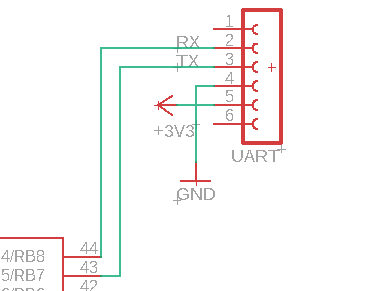
\includegraphics[width=0.8\textwidth]{figures/hardware/UART.PNG}
    \caption{The UART module}
    \label{fig:uart}
\end{figure}

\FloatBarrier
\vspace{1cm}


\subsubsection{Light-emmiting Diodes (LEDs)}

To motivate the use of 2 LEDs in our micromouse, imagine the following: The PCB lies on the 2 wheels, which are screwed on either side somewhere in the middle. Naturally, the PCB will tilt forwards or backwards until it touches the ground, depending on where most weight lies (front sensors). This is highly unwanted: Not only would it result in an unelegant movement creating uneccessary impedance, but the PCB could be potentially damaged by friction and by ground anomalies.

Therefore, for mechanical stability, we use one LED on the front and one on the back of our PCB. They are through-hole components, with the head of the LED resting on the under side of the PCB. The smooth surface of the head works to our favor, not only stabilizing the micromouse, but also offering minimum resistance while moving. The height of the protruding LED head can be decided during soldering according to mechanical needs.

Now, since we have the LEDs, it would be nice to be able to turn them on and off at will. For example we can light the front LED when the micromouse is moving forward and the back one when it's moving backwards.
The sub-circuit for controlling the LEDs can be seen in Fig. \ref{fig:leds}.

\begin{figure}[htb]
    \centering
    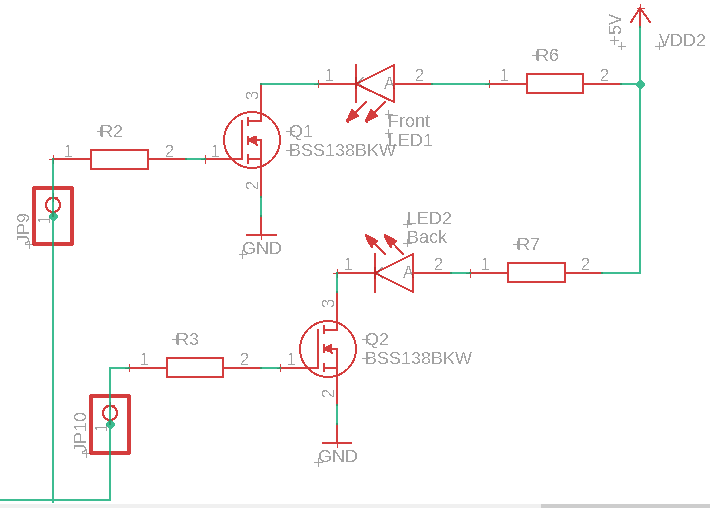
\includegraphics[width=0.8\textwidth]{figures/hardware/LEDs.PNG}
    \caption{The LEDs used for mechanical stability}
    \label{fig:leds}
\end{figure}
\FloatBarrier

The sub-circuits for both LEDs are identical, so let us examine one of them, say the front one. The main component, besides the LED, is an N-channel metal-oxide semiconductor field-effect transistor (MOSFET).

To motivate the need for the MOSFET, imagine connecting the LED directly to the I/O pin. In the datasheet of a typical low current LED (and also the one we will be using) \cite{leds}, we find that the current can be somewhere between 25 - 140 mA. However, the value of 140mA can only be reached under certain PWM conditions. In our case, 20mA steady current will suffice for a bright enough LED. Also the voltage drop on the LED is 2.2 - 2.5V for $I = 20mA$.

Remember the electrical characteristics of the mcu pins as presented in Fig. \ref{fig:electrical}. Notice that the limit current per pin is 4mA! In other words, if we directly connect the LED to the mcu, we will damage the mcu pin and potentially other parts of the mcu circuit. 
Now, the MOSFET serves as a switch: By providing a low current to its gate (the pin of the MOSFET connected to the mcu pin), its channel between the drain and source opens. in other words, it allows current to flow from the LED side to the ground side, thus closing the circuit and lighting the LED up! 

The resistor R2 in the sub-circuit is used to charge the capacitance of the transistor gate. Hence its value is not critical in our case, since no intense time precision demands are made on the LED. We can use our typical 47k resistors also here. Notice that exactly next to the mcu pin, a header pin is placed with the name JP9. This is just a convenient way to later check the voltage of the pin on the pcb for debugging purposes.


The last component to cover is the resistor on the side of the LED. To choose an appropriate value, we need to consider the voltage drop on the LED. As we read above it's somewhere between 2.2 and 2.5V. We can use $\Omega$mhs law, by considering the resistance of the transistor negligible and the resistance of the diode fixed. For the current flowing, let's choose 20mA as stated above. 

$$V_R = I * R => 5 - V_{diode} = I * R$$

For the values $V_{diode} = 2.2V$ and $I = 20mA$ we acquire a value of 140$\Omega$. So, this is the value we need for the resistor.

\vspace{1cm}

\subsubsection{Oscillator}

%%% Somewhere describe the external oscillator choice, the PLL used, the system frequency.

The external oscillator and its capacitors can be seen in Fig. \ref{fig:oscillator}.

\begin{figure}[htb]
    \centering
    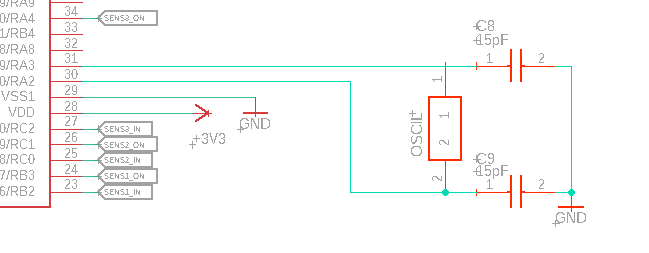
\includegraphics[width=0.8\textwidth]{figures/hardware/Oscillator.PNG}
    \caption{The external oscillator}
    \label{fig:oscillator}
\end{figure}

\FloatBarrier
\vspace{1cm}


\subsubsection{Distance Sensors}

The distance sensors are necessary for perceiving the distance from maze walls. Their sub-circuit can be seen in Fig. \ref{fig:sensors}.

\begin{figure}[htb]
    \centering
    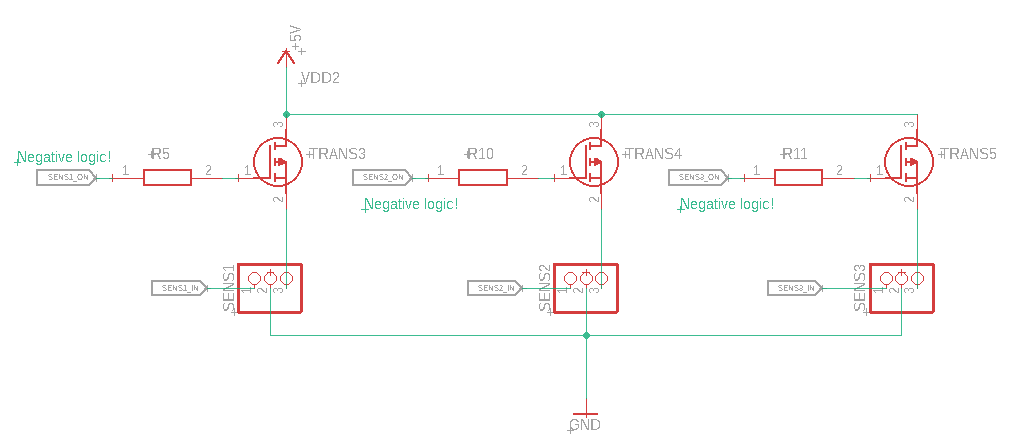
\includegraphics[width=0.8\textwidth]{figures/hardware/DistanceSensors.PNG}
    \caption{The distance sensors}
    \label{fig:sensors}
\end{figure}

\FloatBarrier

To understand their pins, have a look at Fig. \ref{fig:sensorsData} taken from the datasheet \cite{sens}.

\begin{figure}[htb]
    \centering
    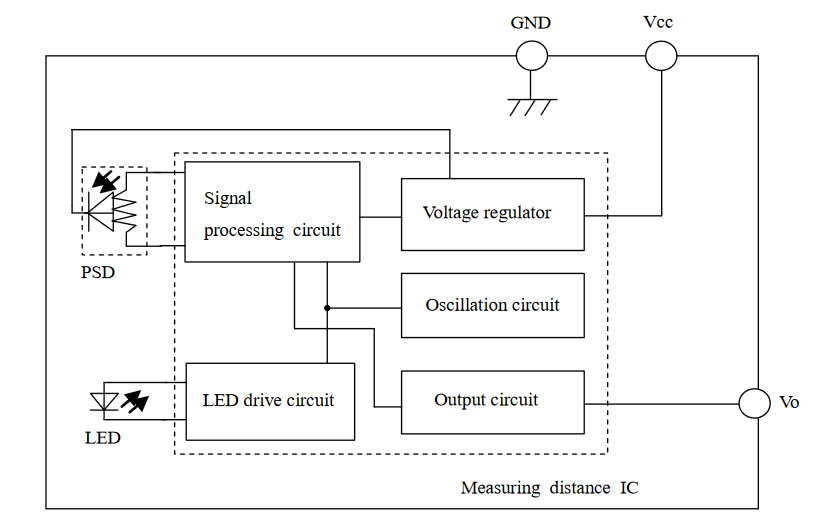
\includegraphics[width=0.8\textwidth]{figures/hardware/sensorData.PNG}
    \caption{Internal schematic of the distance sensors}
    \label{fig:sensorsData}
\end{figure}
\FloatBarrier

Instead of connecting the voltage feed directly to 5V, we use a P-channel MOSFET to turn the sensors on and off at will. The connection of the transistor is the opposite of the N-channel described above (Section LEDs) and its functionality is the same: It is used as a switch. Notice the 47k resistors that connect the gates of the transistors to the pins of the mcu. By offering current from the pins, we close the switch and activate the sensors. Being able to turn the sensors on and off mostly offers flexibility in software.

Last, we feed the incoming data from the sensors to dedicated analog pins in our mcu.

\vspace{1cm}


\subsection{Components}

In this section, just for reference, we list the actual components we chose to order. Most of the components were ordered from \textit{RSComponents}, Fig. \ref{fig:compRS} and the rest from \textit{Mouser}, Fig. \ref{fig:compMou}. The purpose of the lists provided are simply for reference. The components chosen are not unique. Also, the choice of supplier was mostly made due to component availability reasons.

\begin{figure}[htb]
    \centering
    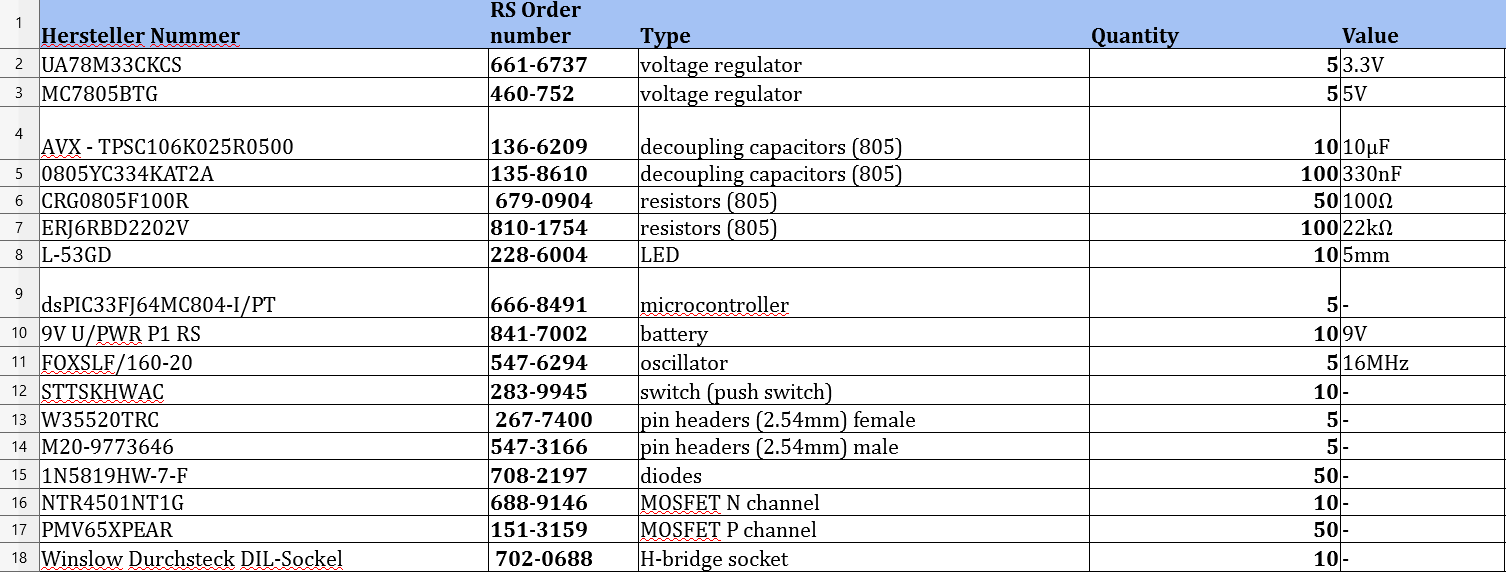
\includegraphics[width=1\textwidth]{figures/hardware/Components1.PNG}
    \caption{List of components ordered}
    \label{fig:compRS}
\end{figure}


\begin{figure}[htb]
    \centering
    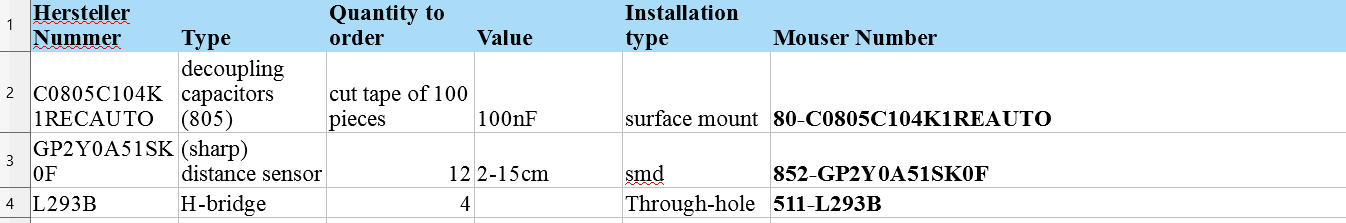
\includegraphics[width=1\textwidth]{figures/hardware/Components2.PNG}
    \caption{List of components ordered (cont.)}
    \label{fig:compMou}
\end{figure}
\FloatBarrier

Notice that the quantities mentioned are not referring to one board only. The quantities ordered were chosen with the thought of building 4 PCBs, checking the availability of existing components in the lab and the minimum components order of the suppliers. 
For the number of components needed per board, please refer to the Schematic and Fig. \ref{fig:comp1} and \ref{fig:comp2}.

\begin{figure}[htb]
    \centering
    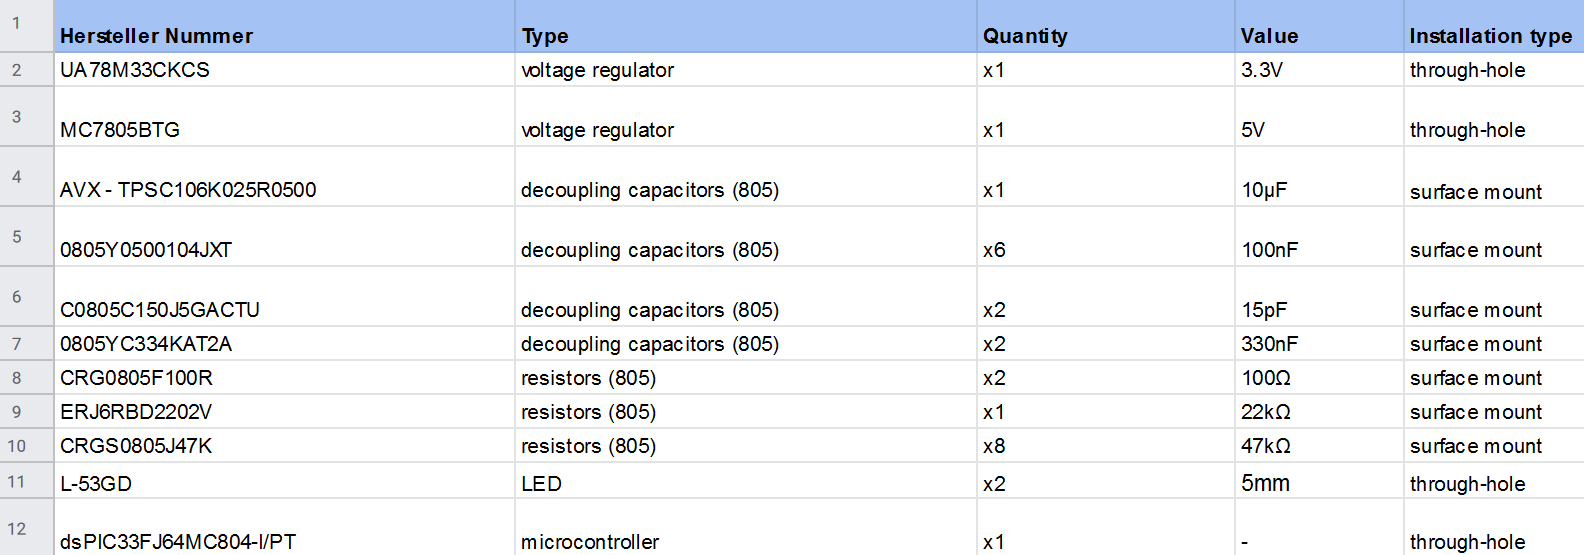
\includegraphics[width=1\textwidth]{figures/hardware/CompList.PNG}
    \caption{List of components needed for one PCB}
    \label{fig:comp1}
\end{figure}


\begin{figure}[htb]
    \centering
    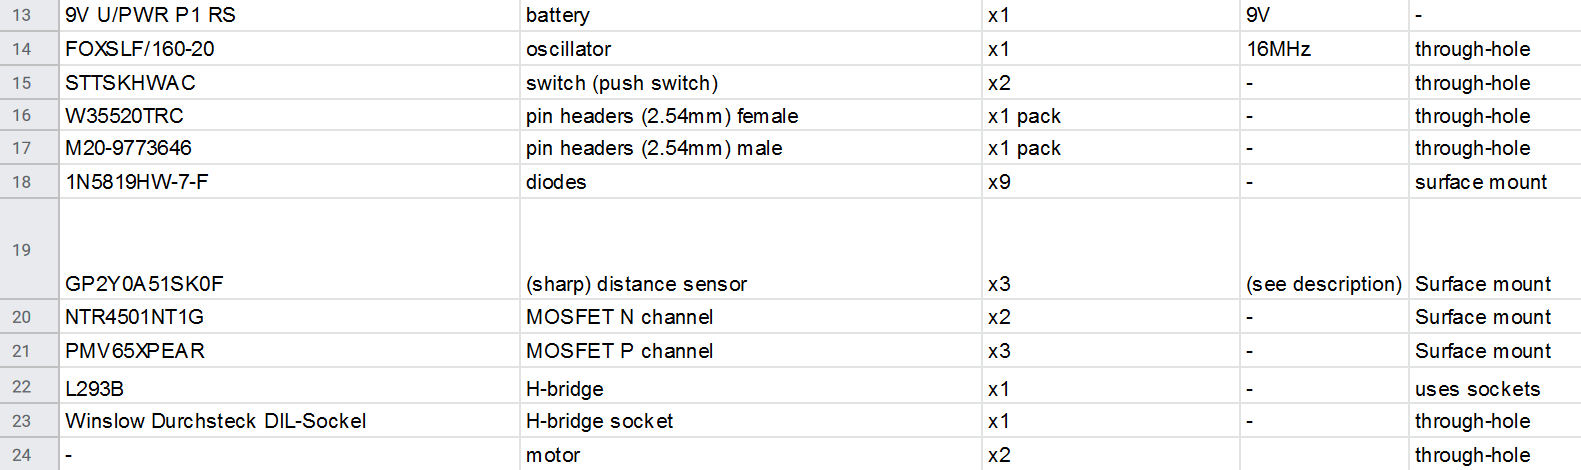
\includegraphics[width=1\textwidth]{figures/hardware/CompList2.PNG}
    \caption{List of components needed for one PCB (cont.)}
    \label{fig:comp2}
\end{figure}
\FloatBarrier

\vspace{1cm}


\subsection{Printed Circuit Board (PCB)}

Comment on the restrictions of the PCB, dimensions and shape.
Explain the components' placement choice.
Describe the concept of 2 layers and via points.
Describe the concept of ground plane.
Comment on electrical noise, its sources and why it doesn't really matter in our case.
Explain the track size chosen.

In this chapter, the PCB of the micromouse will be presented. All in all, the PCB is the body and soul of the robot: Its physical aspect constitutes the largest part of the robot and hosts the mcu (the brain of the robot) and all the necessary components already described in Schematic Section. 

The connections between components are made with tracks of copper running through the PCB. It can be easily seen that the dimensions of the PCB are a trade-off between comfort and practicality: The larger the PCB, the more spacious, the easier it is to solder components on it and design easily distinguishable tracks. The smaller it is the smaller and lighter the robot. In our case the dimensions of the PCB are 
%%% Measure dimensions properly.

Notice that in our case, a 2 layer PCB is designed. The top and bottom layers, both contain components. To fully appreciate this fact, keep in mind that there are 2 different kinds of components used on a PCB: Through-hole and surface mount (SMD). 

The through-hole components actually go through the PCB. The manufacturer needs to drill holes for this purpose. An advantage of this type is mechanical stability. Another advantage comes in the tracking phase, when connecting the components: The through-hole ones can have tracks leading to and from them in both the top and bottom layers. The reason is obvious, they have physical presence in both layers, since they go through the surface of the PCB to the other side. However, the whole concept does occupy more space than the SMD components. Also, drilling holes costs more on the side of the manufacturer.

Now the SMD components are soldered only on the surface of the PCB (top or bottom layer) and no drilling is required. They occupy less space too. However, a track can lead to or from them only in the layer they are found. If a connection between SMD components in different layers needs to be made, a change of layer on the track is necessary, somehwere in its course.

Such changes are accomplished through the so-called "via points".


\begin{figure}[htb]
    \centering
    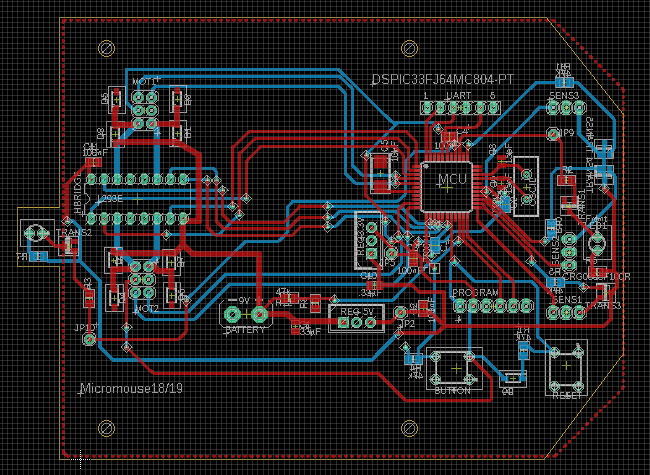
\includegraphics[width=0.8\textwidth]{figures/hardware/PCB.PNG}
    \caption{The PCB with both top and bottom tracks visible}
    \label{fig:pcb}
\end{figure}

\begin{figure}[htb]
    \centering
    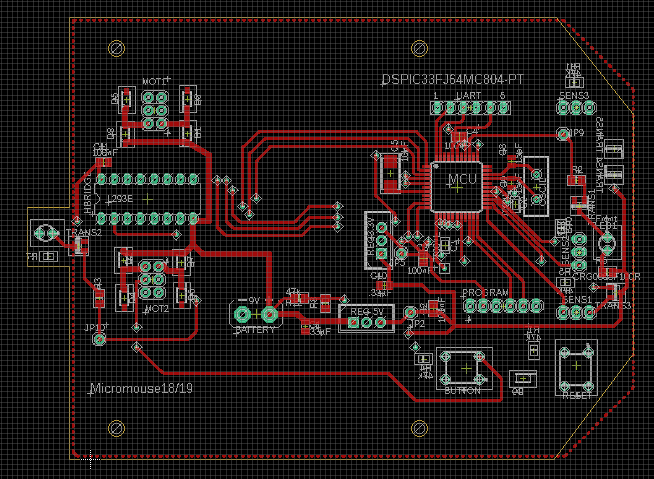
\includegraphics[width=0.8\textwidth]{figures/hardware/PCB_Top.PNG}
    \caption{The PCB with only top layer tracks visible}
    \label{fig:top}
\end{figure}

\begin{figure}[htb]
    \centering
    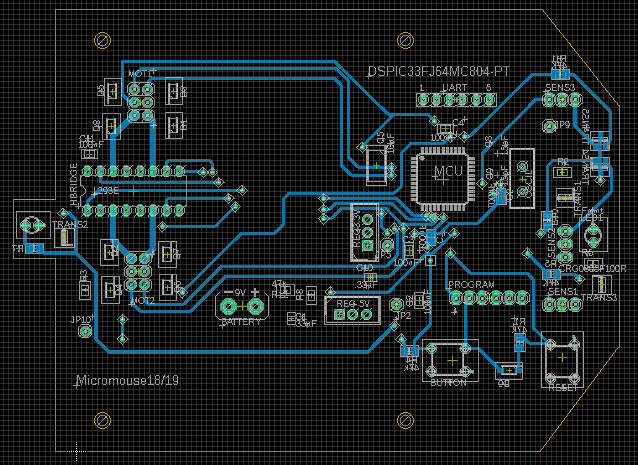
\includegraphics[width=0.8\textwidth]{figures/hardware/PCB_Bottom.PNG}
    \caption{The PCB with only bottom layer tracks visible}
    \label{fig:bottom}
\end{figure}

\begin{figure}[htb]
    \centering
    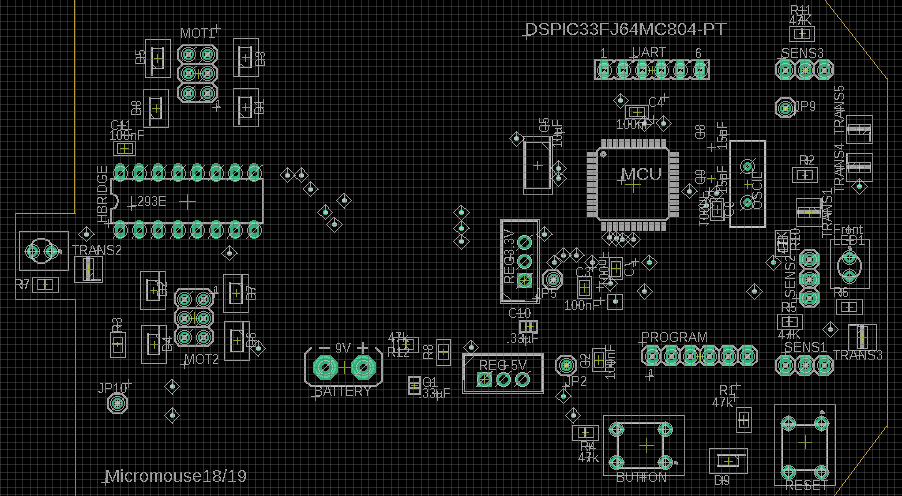
\includegraphics[width=0.8\textwidth]{figures/hardware/PCB_Components.PNG}
    \caption{The PCB without tracks, only components visible}
    \label{fig:comp}
\end{figure}

\begin{figure}[htb]
    \centering
    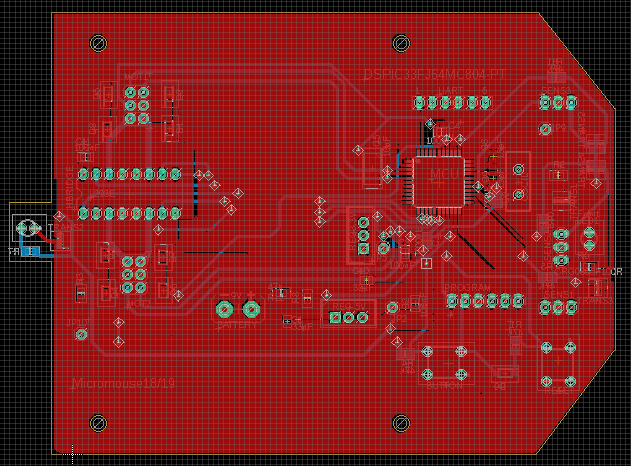
\includegraphics[width=0.8\textwidth]{figures/hardware/PCB_Grounded.PNG}
    \caption{The PCB with the ground plane visible}
    \label{fig:gnd}
\end{figure}

\FloatBarrier

\subsection{Casing}

Present the need for casing.
Describe it.
Present necessary pictures.
Describe important calculations.






